Opampens forsterkning begrenses av høy frekvens.
Et Bode-diagram viser sammenhengen mellom fekvens og forsterkning.
\\\\
Signalet til en opamp blir også faseforskjøvet etter som frekvens endrer seg.
For hver 2. dekade blir signalet forskjøvet med 90°.

\begin{figure}[H]
  \caption{Forhold mellom forsterkning/fase og frekvens}
  \centering
  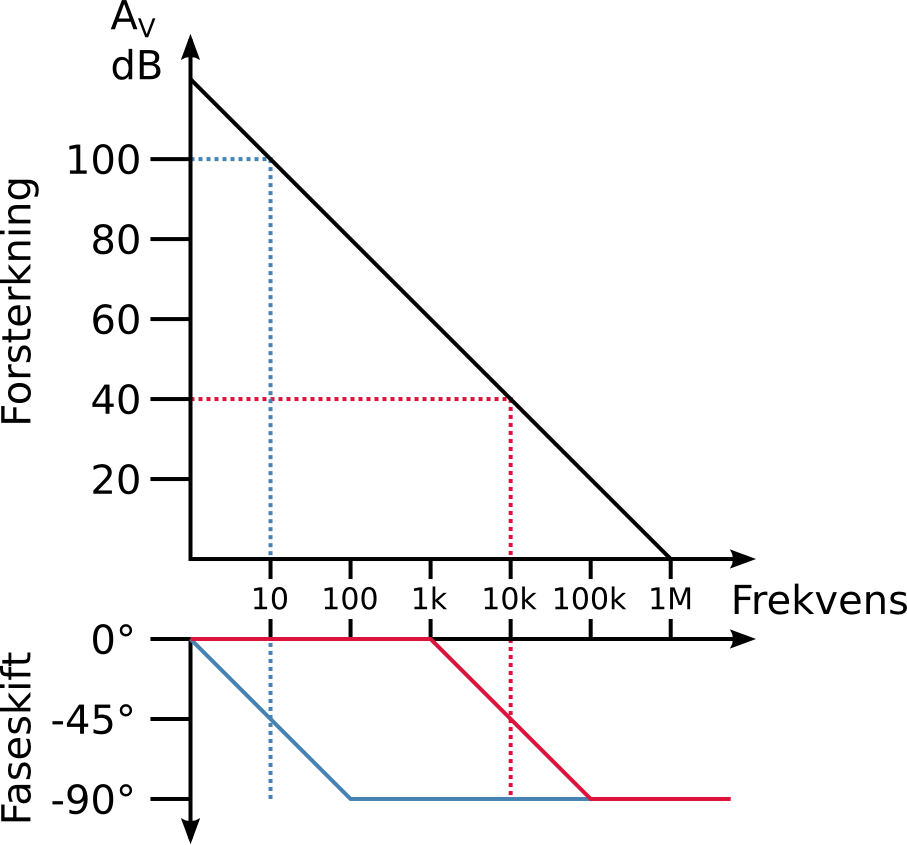
\includegraphics[width=0.67\textwidth]{./img/frekfor}
\end{figure}

Båndbredden er avhengig av hvilken forsterkning vi ønsker.
F.eks. vil $A_v = 40dB$ gi en øvre grense på 10kHz.
Og forsterkning på 20dB har øvre grense på 100kHz.
\\\\
Ved grensefrekvensen forekommer et faseskifte.
Som man kan se begynner det én dekade før og ender én dekade etter.
Totalt 90° forskyvning.



\paragraph{Gain-Bandwidth Product} \mbox{} \\
Gain-Bandwidth Product, GBW, bestemmer skråningen på grafen over.
Produsenter oppgir GBW ved $A_v = 1$, altså der grafen treffer x-aksen.
\\\\
Eksempel\\
$$GBW = A_v \cdot B_w$$
La oss si at $GBW = 1MHz$ og vi ønsker forsterkning på $A_v = 100$.
$$BW = \frac{1MHz}{100} = 10kHz$$
